%!TEX root = thesis.tex

\chapter{Aufbau der Materie}
\label{chapter-materie}

\begin{displayquote}
\begin{center}
\textit{Daß ich nicht mehr mit sauerm Schweiß,\\
Zu sagen brauche, was ich nicht weiß;\\
Daß ich erkenne, was die Welt\\
Im Innersten zusammenhält}
\end{center}
\begin{flushright}
\textit{Faust}, J. W. von Goethe
\end{flushright}
\end{displayquote}

\section{Woraus besteht das Universum?}

Das Universum wird in der Regel beschrieben als endlicher aber unbeschränkter Raum oder Bereich, in dem sich alle uns zugänglichen dinglichen und nicht-dinglichen Phänomene befinden.

Diese Aussage ist nach unserem Wissen richtig, aber auch verhältnismäßig inhaltsleer. Die Realität ist, dass wir nicht wissen was genau das Universum ist, worin es seinen Ursprung hat, und warum es so funktioniert wie es funktioniert. 

Wir wissen allerdings inzwischen mit relativ großer Genauigkeit, wie es funktioniert, das heißt wir können viele (aber nicht alle) Phänomene im Universum erklären und auch voraussagen. Dieses Erklären und Voraussagen ist die Domäne der Naturwissenschaften und im Speziellen der Physik. Alle anderen Naturwissenschaften können prinzipiell als Spezialisierungen der Physik auf Teilbereiche der Naturwissenschaft angesehen werden.

Aus Sicht der klassischen Physik können die uns bekannten Phenomene in zwei Gruppen aufgeteilt werden: \textit{Materie} und \textit{Kräfte}, die wir im Folgenden betrachten wollen.

\section{Materie}
\lipsum[1]
\section{Kräfte}
Wie wissen jetzt, woraus Materie besteht. Aber wie interagiert Materie miteinander? Die Phenomene, welche bei der Interaktion von Materie miteinander oder bei Veränderung der Materie auftreten, fasst man unter den Begriffen \textit{Wechselwirkungen} oder \textit{Kräfte} zusammen. Zu jeder Kraft gehört ein Überträgerteilchen, welches die Wirkung der Kraft vermittelt.

Grundsätzlich sind uns vier Wechselwirkungen bekannt.

\subsection{Die elektromagnetische Kraft}


Die Elektromagnetische Wechselwirkung wirkt zwischen elektrisch geladenen Teilchen. Ihre für uns sichtbaren Ausprägungen sind die elektrostatische Anziehung und Abstoßung, sowie die magnetische Anziehung und Abstoßung, die beide Formen der gleichen Kraft sind. Das Überträgerteilchen der elektromagnetischen Kraft ist das Photon, welches auch einzeln existieren kann.

Die elektromagnetische Kraft hat vermutlich mit den größten Einfluss auf unser Leben, sie ist dafür verantwortlich, dass feste Gegenstände nicht durcheinander hindurch fallen können, die ist eine der Treibenden Kräfte hinter chemischen Reaktionen, und ihr Überträgerteilchen, das Photon, durchdringt unser Leben in Form von Radiowellen, Licht, Röntgen- und Gammastrahlen, die alle elektromagnetische Strahlung verschiedener Frequenzen sind.

Die Reichweite der elektromagnetischen Kraft ist unbeschränkt.

Die Ausprägung als elektrostatische Kraft wird durch das Coulomb-Gesetz beschrieben:
\begin{eqnarray}
 F_C=\dfrac{1}{4\cdot\pi\cdot\epsilon_0}\cdot\dfrac{q_1\cdot q_2}{r^2}
 \end{eqnarray}
Dabei ist $\pi=3,1415...$ die Kreiszahl, $\epsilon_0=8,854188\cdot 10^{-12} \dfrac{A\cdot s}{V\cdot m}$ die elektische Feldkonstante, $q_1$ und $q_2$ die Ladungen der betrachteten Punktladungen in Coulomb (Abgekürzt C, als zusammengesezte Einheit Ampere mal Sekunde), und r der Abstand der Ladungen in Meter.

Die Kraft in der Ausprägung als Magnetismus bezeichnet man als magnetische Kraft:
\begin{eqnarray}
\vec{F}_B = q \cdot \vec{v} \times \vec{B}
\end{eqnarray}
$q$ ist dabei die Ladung in Coulomb die sich mit der Geschwindigkeit $\vec{v}$ (in Meter pro Sekunde) durch ein Magnetfeld der magnetischen Flussdichte $\vec{B}$ (Einheit Tesla, abgekürzt $T=\dfrac{kg}{A\cdot s^2}=\dfrac{V \cdot s}{m^2}$). Das $\times$ bezeichnet die mathematische Operation des Kreuzproduktes.

Zusammen bezeichnet man die Summe aus diesen beiden Kräften als Lorenzkraft

\begin{eqnarray}
\vec{F}_L=\vec{F}_C+\vec{F}_B
\end{eqnarray}


Um Verwirrung zu vermeiden ist dabei ist aber zu beachten, dass in älteren Lehrbüchern abweichend davon die magnetische Kraft $\vec{F}_B$ als Lorenzkraft $\vec{F}_L$ bezeichnet wird.  



\subsection{Die kernstarke Kraft}

Die kernstarke Kraft ist für den Zusammenhalt der Quarks, und damit der aus den Quarks gebildeten Baryonen Proton und Neutron, sowie aller anderer in der Natur normalerweise nicht frei vorkommenden aus Quarks gebildeten Teilchen (Hadronen) verantwortlich. Sie vermittelt ebenso den Zusammenhalt benachbarter Hadronen, insbesondere in Atomkernen den Zusammenhalt zwischen Protonen und Neutronen im Atomkern. 

Die Überträgerteilchen der kernstarken Kraft sind die Gluonen, von denen es 6 verschiedene Ausprägungen sowie nochmals genausoviele Antiteilchen dazu gibt.

Die Reichweite der kernstarken Kraft ist sehr klein, und liegt im Bereich des Durchmessers eines Atomkerns. Dafür ist aber ihre Energie sehr hoch. In der Regel spielt die kernstarke Kraft in unserem Alltag keine große Rolle. Die Änderung des Bindungszustandes der kernstarken Kraft in Atomkernen bei radioaktivem Zerfall, Kernspaltung und Kernfusion ist aber für die dabei frei werdenden Energiemengen verantwortlich, so dass insbesondere Kernkraftwerke sowie nukleare Waffen ohne sie nicht möglich wären.

Die Berechnung der kerstarken Kraft ist mit Rechnungen der klassischen Physik nicht möglich, dazu werden Rechenmethoden der Quantenchromodynamik und der Quantenfeldtheorie benötigt, welche den Umfang dieser Vorlesung bei weitem überschreiten, und deshalb hier nicht ausgeführt werden sollen. Bei Interesse sei auf Lehrbücher zu diesen Berechen der Physik verwiesen.

\subsection{Die kernschwache Kraft}

Die kernschwache Kraft vermittelt zwei der fünf bekannten Radioaktiven Zerfallsarten, den $\beta^+$- und den $\beta^-$-Zerfall, ausgesprochen als \textit{Beta Plus} bzw. \textit{Beta Minus}.

Ihre Überträgerteilchen sind das $W^+$-, das $W^-$-, sowie das neutrale $Z$-Boson, die alle eine sehr kurze Reichweite aber eine große Masse haben

Dabei zerfällt beim $\beta^-$-Zerfall ein down-Quark in ein up-Quark und ein $W^-$-Boson. Letzters zerfällt dann kurze Zeit später in ein Elektron und ein Elektronen-Antineutrino. Durch die Umwandlung des down- in ein up-Quark wandelt sich das Neutron, in dem sich das Quark befindet in ein Proton um.

Analog dazu zerfällt beim $\beta^+$-Zerfall ein up-Quark in ein down-Quark und ein $W^+$-Boson. Letzters zerfällt dann kurze Zeit später in ein Positron (Antielektron) und ein Elektronen-Neutrino. Durch die Umwandlung des up- in ein down-Quark wandelt sich das Proton, in dem sich das Quark befindet in ein Neutron um.

Genau wie die kernstarke Kraft kann auch die kernschwache Kraft nur mit Methoden der Quantenchromodynamik und der Quantenfeldtheorie berechnet werden. Daher gilt das oben gesagte hier ebenso.

\begin{figure}
    \centering
    \def\svgwidth{\columnwidth}
    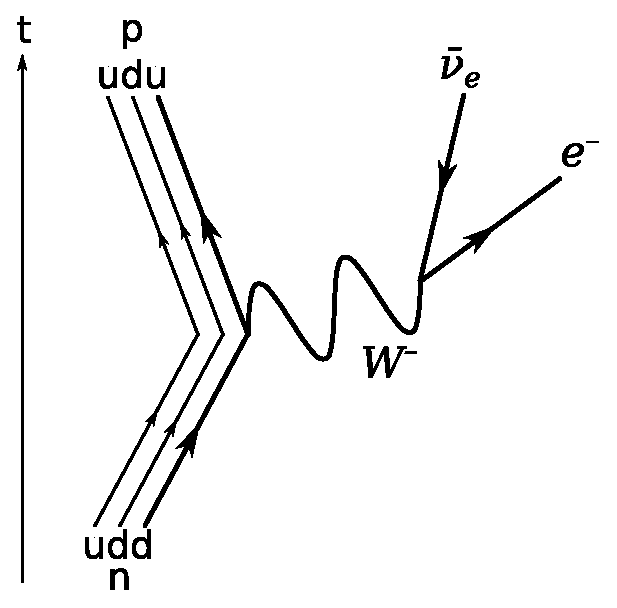
\includegraphics[scale=0.5]{Beta_Negative_Decay.eps}
    \caption{$\beta^-$-Zerfall im Feynmanndiagramm} 
\end{figure}

\subsection{Die Gravitationskraft}

Die Gravitationskraft fällt in der Gruppe der Kräft etwas aus der Reihe, da weder ihre Ursache noch das vermittelne Teilchen bisher sicher bekannt sind. Nach der Relativitätstheorie ist die Gravitation keine Kraft welche wie die anderen Kräfte durch ein Teilchen vermittelt wird, sondern eine Eigenschaft des Raumes, der durch seine Form die Masseteilchen beeinflusst. Es wird aber auch vermutet, dass es trotzdem ein Gravitationsteilchen, das Graviton, geben muss. Dieses wurde bisher aber nicht gefunden. Siehe dazu auch \ref{chapter-qmrt}.

Die Gravitation hat wie die elektromagnetische Kraft eine unbeschränkte Reichweite, ist jedoch um etliche Größenordnungen schwächer als diese oder die anderen beiden Kräfte. Der Grund für diesen extremen Unterschied ist ebenfalls nicht bekannt und Gegenstand der Forschung.

Die Gravitationskraft kann mit folgender Formel berechnet werden
\begin{eqnarray}
\vec{F}_G=\dfrac{m_1 \cdot m_2 \cdot G}{\vec{r}^2}
\end{eqnarray}

Dabei sind $m_1$ und $m_2$ die Massen der beiden Objekte die sich anziehen in Kilogramm, $G$ ist die Gravitationskonstante mit dem Wert $G=6,67430\cdot 10^{-11} \dfrac{m^3}{kg \cdot s^2}$, und $\vec{r}$ ist der Abstand der beiden Massen in Meter. Man verwendet dafür den Abstand zwischen dem Massenschwerpunkten, also den mit der lokalen Dichte gewichteten Mitten. In erster Näherung kann dafür auch die geometische Mitte der Massen verwendet werden.

\section{Statistische Thermodynamik}
\lipsum[1]
\section{Übungsaufgaben}
\lipsum[1]